\documentclass[12pt,letterpaper]{article}
\usepackage[utf8]{inputenc}
\usepackage[spanish]{babel}
\usepackage[rmargin=2cm,lmargin=2cm,tmargin=3cm,bottom=3cm]{geometry}

\usepackage{fancyhdr}
    \pagestyle{fancy}
        \fancyhf{}
        \rhead{}
        \lhead{}

\usepackage[x11names,table]{xcolor}
\usepackage{graphicx}
\usepackage{caption}
\usepackage[rightcaption]{sidecap}

\usepackage{amsmath}
\usepackage{amssymb}
\usepackage{dsfont}
\usepackage{latexsym}
\usepackage{mathrsfs}

\usepackage{array}
\usepackage{multirow}
\usepackage{multicol}
\usepackage{colortbl}

\usepackage{hyperref}
\hypersetup{colorlinks=true}

\usepackage{blindtext}

\usepackage[backend=biber, citestyle=alphabetic, style=apa]{biblatex}
\bibliography{Bibliografia}
%---------------Pagina 1 (portada)---------
\begin{document}
\begin{center}
    \textsc{\Huge{Universidad Nacional Autónoma de México}}
    \\
\end{center}
\begin{center}
{\textsc{\Huge{Facultad de ciencias}}}
\end{center}
\begin{center}
{\textsc{\Huge{Fisíca}}}
\end{center}
\begin{center}
{\textsc{\Huge{Computación}}}
\end{center}

\begin{center}
\vspace{0.5cm}
    \textcolor{magenta}{\textsc{\Huge{El programa MACTZIL}}}
\end{center}

\begin{SCfigure}[0.999][ht]
\raggedright
     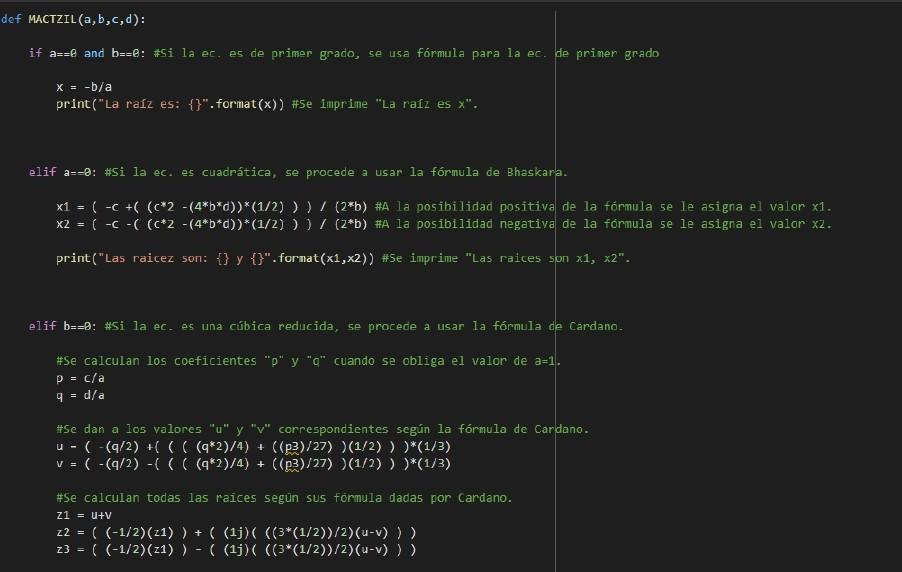
\includegraphics[scale=0.9]{imagenes/p3.jpg}
     \label{fig:my_label} 
\end{SCfigure}
\vspace{0.3cm}
\begin{center}
   \textsc{\Huge{Grupo: 8108 }}
\end{center}
\begin{multicols}{2}
\Large{\textbf{Profesor:}}
	
 Pedro Arturo Flores Silva

\Large{\textbf{Ayudantes:}}

Ivan jiménez Lopéz 

Omar Montoya Trejo	

\Large{\textbf{Integrantes del equipo:}}

Archundia Juárez Adrián

Duarte Martínez Jordán Aarón

Nayeli Rodriguez Vega

\end{multicols}


\newpage
%-----Pagina terminada----

%---------Pagina 1 (Indice)---
\pagestyle{fancy}
        \fancyhf{}
        \rhead{Universidad Nacional Autónoma de México}
        \lhead{MACTZIL}
        \lfoot{Diciembre del 2022}
\begin{center}
    {\textbf{\textsc{\Huge{Indíce}}}}
\end{center}
\begin{enumerate}
\item Resumen...............................................................................................................................3
\item 
Introducción.........................................................................................................................3
\item 
Preludio al programa.........................................................................................................3-5
\item El programa MACTZIL.....................................................................................................5-7
\item Resultados.............................................................................................................................7
\item Conclusiones..........................................................................................................................8
\item Refenrencias..........................................................................................................................8
    
\end{enumerate}
\newpage
%--------------final de la pagina-----------

\pagestyle{fancy}
        \fancyhf{}
        \rhead{Universidad Nacional Autónoma de México}
        \lhead{MACTZIL}
        \lfoot{Diciembre del 2022}
        \rfoot{\thepage}

\section{Resumen}
\noindent El presente trabajo aborda la nesesidad de estudiar sistematicamente y de manera continua el calculo de ecuaciones de segundo y tercer grado con numeros complejos, por medio de un programa hecho en python llamado "El programa MACTZIL" en el cual, nos tubimos que basar en el método de Bhaskara y en el método de Cardano para realizar el programa, igualmente tuvimos que ocupar diversos comando y/o codigos para nos diera un resultado considerable.
\\

\noindent Palabras clave: Ecuaciones, Programació, Método de Bhaskara, Método de Cardano, Programación.
\section{Introdución}

\noindent La resolución de problemas que involucran encontrar un valor desconocido o el valor de una variable apareció hace mucho tiempo, debido a que existe informes del periodo babilonio que tratan del 1700 A.C, en donde nos muestran la solución de problemas que involucran ecuaciones complejas, no obstante en la cultura egipcia también podemos ver en sus papiros como intentaban resolver problemas de ecuaciones, pero no llegaban a un resultado concreto ya que los egipcios obtenía la solución mediante un procedimiento llamado el método de la falsa posición, más tarde este método pasó a los árabes en donde trataban la solución de ecuaciones por simple y doble o falsa posición. Este último procedimiento es similar al actual que es utilizado para resolver ecuaciones no lineales por métodos numéricos, sin embargo, tuvo que pasar un poco menos de 3000 años para encontrar los primeros indicios de las ecuaciones como objetos matemáticos y procedimientos que actualmente conocemos, como el método de Bhaskara (formula general) que es utilizado para resolver ecuaciones de segundo grado o el método de Cardano que es usado para resolver ecuaciones de tercer grado.
\\

\noindent Cuando hablamos de las ecuaciones nos referimos a una igualdad matemática entre dos expresiones algebraicas en las cuales aparecen valores conocidos y otros desconocidos, estos últimos son llamados variables o incógnitas que se llegan a representar por una letra y cuya magnitud puede considerarse a partir de las propiedades matemáticas de la ecuación o través de un sistema de ecuaciones. No obstante, dependiendo de la magnitud que sea la ecuación se puede clasifican en ecuación de primer grado, segundo, tercero, etc. 
\\

\noindent Empero, el objetivo del presente proyecto consiste en resolver ecuaciones de segundo grado y de tercer grado con números complejos a través de nuestro programa llamado MACTZIl. 

\section{Preludio al programa}

\noindent En esta sección del proyecto escrito en cuestión se presenta un breve, pero suficiente, recuento historico que da cabida a entender la importancia de la resolución de ecuaciones cuadráticas y cúbicas que hoy día podrían parecer una parte básica de las matemáticas, pero que sin duda, al igual que todas las bases, es fundamental para construir las grandes estructuras matemáticas que nos han dado acceso a un sin número de comodidades y demás beneficios.
\\

\noindent Durante la mayor parte de la historia del ser humano a los problemas de tipo matemático se les ha concebido de forma geometrica, siendo, por ejemplo, una incognita ``x" imaginada como un recta de largo ``x", que sumada con otra recta de largo 4 da como resultado una recta más grande de largo igual a 8. Con simple algebra se llega a que la solución es que ``x" es igual a 4 también. Análogamente, en las ecuaciones cuadráticas se llegaría a que x al cuadrado representa un área, que sumada a otra área nos da una más grande.
\\

\noindent Esta comprensión de las matemáticas iba de la mano con un uso práctico en el que no tenía sentido que existieran rectas de longitud -5, áreas de -25, o -30 vacas. Por tanto, las restas eran sólo usadas con el fin de obtener resultados positivos. Hubo algunos grupos que llevaron las matemáticas más lejos (chinos, babilonios, persas, árabes, indús, griegos, etc.), y deducieron independientemente números como los enteros, y los racionales en ocasiones, sin embargo, jamás llegaron a ideas que salieran de lo geometrico.
\\

\noindent Hablando en cuanto a la solución de ecuaciones cuadraticas, todos estos grupos susodichos idearon la fórmula de Bhaskara, aunque, debido a su apego geométrico, más bien crearon 6 diferentes ecuaciones básicas para resolver cualquier ecuación cuadrática, siempre dando como resultado números positivos. Las ecuaciones susodichas son expresadas a continuación:

$$ax^{2} = bx\quad ;\quad ax^{2}=c\quad ;\quad ax=c\quad ;\quad ax^{2}+bx=c\quad ;\quad ax^{2}+c=bx\quad ;\quad bx+c=ax^{2}$$

\noindent De igual modo, todas estás civilisaciones intentaron crear una serie de formulas, o una sola, para resolver las ecuaciones cúbicas durante más de 4000 años. El que tuvo más exito entre todos ellos fue Omar Khayyam, de Persia, que logró desarrollar 33 ecuaciones para la resolución o formualción de cúbicas al usar como objeto auxiliar círculos; a pesar de su leve exito, el matemático no terminó por encontrar un método confiable para todo polinomio de este grado.
\\

\noindent No sería hasta que el siglo XVI cuando el matemático profesor en la universidad de Bologna, Italia, Scipione Del Ferro que daría a luz una ecuación para resolver polinomios de grado 3 reducidos, es decir, sin el elemento al cuadrado.
\\

\noindent Contrario a lo que se podría pensar, Del Ferro no hizo público su descubrimiento, pues por aquellas epocas el oficio de matemático se mantenía a partir de la reputación con otros matemáticos, de modo que los miembros de este trabajo se podían para destituir a otro, así que, Del Ferro, al guardar en secreto esta fórmula aseguró su trabajo. Y así seguiría hasta que 20 años después se lo revelaría a su estudiante, Antonio Fior, mientras yacia en el lecho de la muerte.
\\

\noindent Fior era más osado que su predecesor, así que se adueño del descubrimiento, y presumió ser capaz de resolver cúbicas reducidas, sin revelar el cómo, claro. Su audacia se elevó a tales niveles que en 1535 desafió a Tartaglia, un respetado matemático que empezo en la pobreza y de modo autodidacta se hizo una reputación en el área en cuestión.
\\

\noindent Como era costumbre, cada uno le planteo 30 ejercicios a su contricante, y contaban con 40 días para resolver la mayor cantidad posible. como es previsible, Fior reto a Tartaglia con 30 ecuaciones cúbicas reducidas, lo que obligo a este último a llevar a los límites su intelecto con tal de mantener su empleo. Objetivo que cumplio, pues al concebir el monomio al cubo como, redundantemente, un cubo de lados ``x", y al termino de grado uno como un prisma de volumen ``bx", con b como su coeficiente, pudo hacer una serie de transformaciones geométricas que le perimitieron crear un algoritmo capaz de resolver las ecuaciones de grado tres sin termino cuadrático.
\\

\noindent Al final, Tartaglia logró resolver todas las ecuaciónes en un aproxiamdo de 2 horas, mientras que Fior no fue capaz de resolver uno solo de los problemas que se le plantearon; su infundado orgullo lo llevo al abismo. La victoria de Tartaglia se hizo viral para aquellos entonces, a tal punto que un erudito, llamado Cardano, le insitio tanto sobre revelarle su método, que al final el 25 de Marzo de 1539 éste accedio tras serle entregada una cuantiosa cantidad de dinero por parte de Cardano, y que además este último jurará no revelar el secreto.
\\

\noindent Cardano empezó a probar el método con metas más ambiciosa, es decir, resolver un polinomio cúbico, con todo y término al cuadrado. Y a partir de preuba y error dió lugar a un método para reducir cualquier ecuación cúbica a una ecuación cúbica reducida, que puede ser resuelta facilmente con el algoritmo de Tartaglia.
\\

\noindent El erudito estaba emocionado y muy tentado a publicar su descubrimiento, pues a diferencia de sus predecesores en la inovación de polinomio de grado tres, el se mantenía con su trabajo de médico; aunque, a pesar de su entusiamos, su promesa a Tartaglia lo mantenía con las manos atadas... Hasta que en 1542 el visitó a un matemático en Bologna, el cual de pura suerte resulto ser el sobrino de Del Ferro. De este modo, mientras que Cardano ojeaba los libros del fallecido erudito, notó que en uno de ellos estaba redactada la misma fórmula que dedujo Tartaglia.
\\

\noindent Teniendo como excusa el descubrimiento previo de Del Ferro, Cardano publicó 3 años después el algoritmo para resolver las cúbicas completas y reducidas en su libro ``Artis Magna". Empero, aquí no acaba la historia, pues como consecuencia de esta publicación el ingeniero Bombelli encontró que para algunas soluciones aparecían raíces negativas, que al operarlas en cierto casos se cancelaban y daban lugar a una solución sin estas raíces; así, Bombelli demonio a este tipo de números como un nuevo tipo de número al no poder ser considerado como negativo o positivo. Años después el matemático Descartes los denominaría con el nombre de imaginarios, y el afamado Euler los denotaría con la letra ``i".
\\

\section{El programa MACTZIL}

\noindent Éste consiste de usar la palbra reservada ``def", de Python, para establecer una nueva función llamada con la palabra ``MACTZIL(a,b,c,d)", en la cual se establecen 4 variables, todas para los coeficientes del posible polinomio $ax^{3}+bx^{2}+cx+d=0$. A partir de ésto la función evalua el valor de los coeficientes en 4 condiciones, las cuales dan lugar a 4 operaciones diferentes para la resolución del polinomio en cuestión.
\\

\noindent A continuación se exponen las 4 condiciones, en orden de aparición en el código, y el procedimiento al que dan lugar una vez que se cumplen.

\begin{enumerate}
    \item Si a=0 y b=0.\\
    
    Al cumplirse esta condición se concluye que el polinomio en cuestión es de grado 1, y por tanto se usa la formula para su resolución, es decir: $x=-d/c$ (con los valores que tendría esta ecuación en cuestión). Tras lo anterior se imprime en la pantalla la solución para el polinomio.
    
    \item Si no se cumple lo anterior, y a=0.\\
    
    Como consecuencia del cumplimiento de esta condición se obvia que la ecuación es cuadrática, y por ello se usa la fórmual de Bhaskara (expuesta debajo de este parrafo) para su resolución, y futura impresión en pantalla de las dos soluciones.
    
    $$x_{1,2} = \frac{-b\pm \sqrt{b^{2} -4ac}}{2a}$$
    
    \item Si no se cumple el anterior, y b=0.\\

    Se deduce que el polinmio en cuestión es una cúbica reducia, por lo que se procede a divir los coeficientes entre el valor del coeficiente de la variable cúbica ($p=c/a\quad ;\quad q=d/a$) para así poder usar el método de Cardano para la resolución de este tipo de ecuaciones, el cual es:
    
    $$u = \sqrt[3]{-\frac{q}{2} +\sqrt{\frac{q^2}{4} + \frac{p^3}{27} } } $$
    $$v = \sqrt[3]{-\frac{q}{2} -\sqrt{\frac{q^2}{4} + \frac{p^3}{27} } } $$

    $$ z_1 = u+v $$
    $$ z_{2,3} = \left[ -\frac{1}{2}(u+v) \right] \pm \left[\frac{\sqrt{3}}{2}(u-v) \right]i$$

    Con z1, z2 y z3 como raíces del polinomio en cuestión que serán impresas en la pantalla.
    
    \item Si no se cumple ninguno de las anteriores condiciones.\\

    El polinomio es una ecuciación cúbica completa, por lo que se opera el método de Cardano para reducción a cúbica reducida con coeficientes 1, p y q (término cúbico, término de grado uno, y término independiente, correspondientemente), para así usar la resolución de Cardano de este tipo de cúbicas. A continuación, sus ecuaciones respectivas en el programa MACTZIL. 

    $$p = \frac{3ac-b^2}{3a^2}$$
    $$q = \frac{2b^{3}-9abc+27a^{2}d}{27a^3}$$
    
    $$u = \sqrt[3]{-\frac{q}{2} +\sqrt{\frac{q^2}{4} + \frac{p^3}{27} } } $$
    $$v = \sqrt[3]{-\frac{q}{2} -\sqrt{\frac{q^2}{4} + \frac{p^3}{27} } } $$

    $$ z_1 = u+v -\frac{b}{3a}$$
    $$ z_{2,3} = \left[ -\frac{1}{2}(u+v) -\frac{b}{3a} \right] \pm \left[\frac{\sqrt{3}}{2}(u-v) \right]i$$

    Con z1, z2 y z3 como raíces del polinomio en cuestión que serán impresas en la pantalla.
    
\end{enumerate}

\section{Resultado}
\noindent Logramos obtener un código nos permite conocer de forma inmediata los resultados de ecuaciones cuadráticas o cubicas, asimismo, si el resultado arroja una solución compleja, lo resuelve por igual.  También es importante recalcar que el código es capaz de resolver la ecuación sin que esta completa, también selecciona automáticamente el método o la vía por donde va a resolver la ecuación, dependiendo del tipo de ecuación en cuestión. Sin embargo, es importante mencionar que posiblemente por defectos de aproximación del sistema operativo, o quizás por la naturaleza de la formula usada para la resolución de ecuaciones cúbicas, hay ocasiones en las que la calculadora no arroja resultados correctos, siendo en su mayoría aproximaciones buenas, y en ocasiones completos errores
\section{Conclusión}
\noindent El código puede ser de gran ayuda, ya que, hace la función de una calculadora, en donde obtienes resultados de polinomios no triviales muy fácilmente, y este puede ser empleado en distintos campos donde se haga uso de el, haciendo que el trabajo de dichas ecuaciones sea mas sencillo y que de esta forma, ayude a la eficacia de trabajos y/o proyectos. 

\section{Referencias}

\begin{itemize}
    \item Ecuación. (s. f.). Significados. https://www.significados.com/ecuacion/
    \item Sobre el origen de las ecuaciones. (s. f.). Junta de extremadura.
    \item Veritasium en español. (12 de diciembre de 2021). Cómo se Inventaron los Números Imaginarios [Video]. YouTube. https://www.youtube.com/watch?v=VN7nipynE0c
\end{itemize}

\end{document}
